\chapter{Rozdział 2}
\section{Przypadki użycia}
Poniżej zostały przedstawione przypadki użycia które użytkownicy mogą podjąć w systemie. Przypadki użycia zostały pogrupowane na podstawie 4 rzeczy: zakładania konta, logowania, zarządzania loterią oraz zarządzania sprzętem komputerowym.

\section{Założenie konta pracowniczego}
Pracownik jest osobą pracującą w firmie.Jako że implementowany system jest niezależny od wewnętrznych systemów firmy potrzebne jest założenie kont dla użytkowników. Użytkownik sam zakłada konto do czego wykorzystuje swojego maila firmowego gdzie można potwierdzić jego tożsamość.

\begin{figure}[h]
    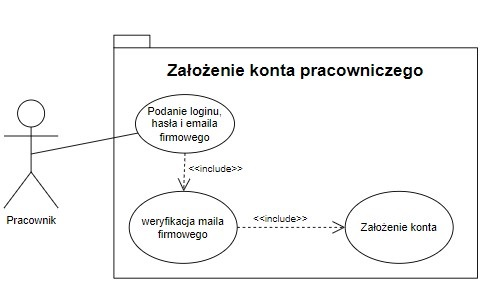
\includegraphics{rys01/zakladanie.jpg}
    \caption{Przypadek zakładania konta pracowniczego}
    \label{zakładanie_konta_etykieta}
\end{figure}

Załączony rysunek Rys.~\ref{zakładanie_konta_etykieta} pokazuje proces rejestracji. Użytkownik najpierw podaje swoje dane. Następnie jeżeli dane są prawidłowe klika w link weryfikacyjny na maili i następuje założenie konta.

\section{Logowanie się do systemu}

\begin{figure}[h]
    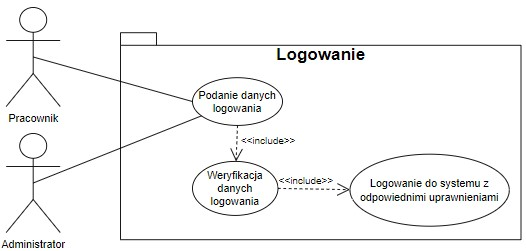
\includegraphics{rys01/logowanie.jpg}
    \caption{Logowanie do systemu z odpowiednimi uprawnieniami}
    \label{logowanie_etykieta}
\end{figure}

W załączonym rysunku Rys.~\ref{logowanie_etykieta} został pokazany proces logowania z odpowiednimi uprawnieniami. Uprawnienia są nadawane na podstawie roli którą pełni użytkownik czyli Pracownik lub Administrator. Uprawnieniami pracownika są: przeglądanie dostępnych loterii, zapisywanie i wypisywanie się z udziału z loterii Rys. ~\ref{loteria_etykieta} Administrator jest osobą zarządzająca loteriami i losowanym sprzętem. Nie może jednak on sam się zapisywać na loterie z konta administracyjnego.
\newpage
\section {Loteria}

\begin{figure}[h]
    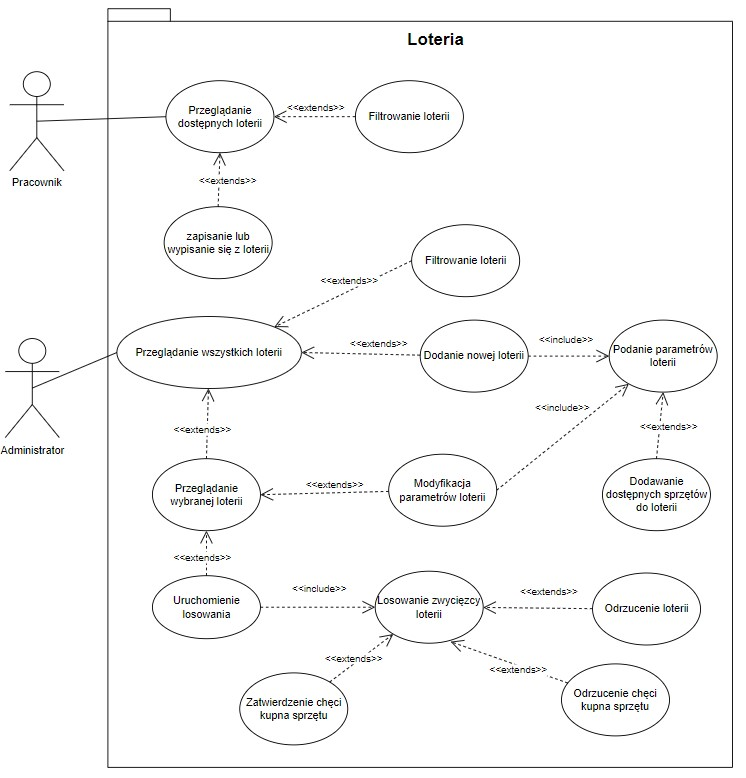
\includegraphics[scale=0.8]{rys01/loteria.jpg}
    \caption{Loteria}
    \label{loteria_etykieta}
\end{figure}


W załączonym rysunku Rys.~\ref{loteria_etykieta} opisywany jest przypadek loterii. Pracownik ma tylko wgląd w aktywne loterie. Może je pofiltrować tak aby były wyświetlane tylko te loterie w których bierze udział lub te w których nie bierze udziału. Ma też możliwość zapisania lub wypisywania się z loterii. W informacjach dotyczących loterii znajdują się informacje dotyczące sprzętu, biura z którego można odebrać sprzęt oraz data losowania. Administrator również może przeglądać loterie. Ma on uprawnienia do edycji i dodawania nowych loterii. Jedna loteria dotyczy jednego sprzętu dlatego równolegle może odbywać się wiele loterii. Pozwala to uniknąć sytuacji kiedy pracownik wylosowałby sprzęt który go nie interesuje. Administrator może ustalić datę losowania. Dla lepszej wygody tworzenia losowań istnieje w systemie funkcjonalność która umożliwia tworzeniu wielu losowań na raz. Gdy wylosowany zostanie zwycięzca który jest pracownikiem może on zatwierdzić lub odrzucić swoją wygraną. W przypadku braku potwierdzenia po określonej liczbie dni loteria może zostać uruchomiona ponownie z tymi samymi parametrami.

\section {Sprzęt komputerowy}

Istotną część w systemie zajmuje sprzęt komputerowy. System wspomaga monitorowanie stanu urządzeń takich jak komputery, stacje dokujące czy tabletu. W przypadku kiedy firma chciała by wystawić na sprzedaż inny sprzęt istnieje specjalna tabela w bazie danych odpowiadająca podstawowemu sprzętowi komputerowemu która jako atrybuty ma podstawowe informacje. Sprzęt w bazie danych jest już oddany do odsprzedaży, należy zrobić jego wycenę i podać jego parametry.

\begin{figure}[h]
    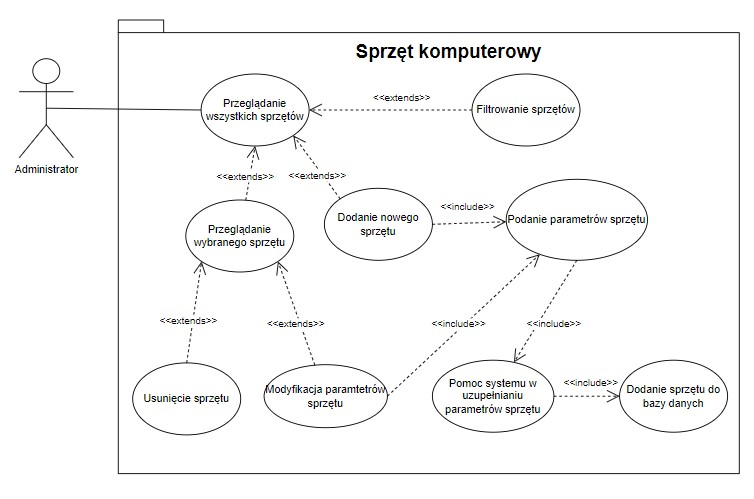
\includegraphics[scale=0.8]{rys01/sprzet.jpg}
    \caption{Sprzęt komputerowy}
    \label{sprzet_etykieta}
\end{figure}


W załączonym rysunku Rys. \ref{sprzet_etykieta} Jedyną osobą która może zarządzać sprzętem jest administrator. To on dodaje sprzęty do bazy danych przez aplikacje, z tym że system pomaga mu podpowiadając pola takie jak procesor, pamięć i pamięć RAM. System także pomaga oszacować cenę urządzenia na podstawie zaimplementowanego algorytmu szacowania ceny, z tym że ostateczna cena urządzenia jest podawana przez administratora. Pracownik może przeglądać urządzenia i jego parametry ale z poziomu loterii Rys.~\ref{loteria_etykieta}





